
	\newpage
% =========================================================
	\section{Quadratur}
% =========================================================

	\defi{
		\n 
		Nachdem wir herausgefunden haben, wie wir eine Funktion mithilfe von Interpolation annähern können, drängt sich sofort die Frage auf, wie das mit der Integration einer Funktion aussieht.
		\n
		Es geht nicht nur, sondern auch noch recht simpel. Wir interpolieren die Funktion mithilfe von schon besprochenen Methoden und integrieren dann einfach analytisch. So integrieren wir eine Annäherung der Funktion und erhalten damit auch eine Approximation des Integrals. Dies ist die Kategorie der Quadratur-Probleme.
	}

	\sbreak
	\methode{ \label{sec:quadratur_regeln}
		\n 
		Allgemeines Quadraturproblem: 
		\begin{align*} 
 			\int_{a}^{b}f(x)\d x \approx \sum_{i=1}^{n}f(x_i) \cdot w_i 
 		\end{align*}
 		Die $w_i$ nennt man Gewichtungen, also wir gewichten $f(x_i)$ Werte, die ja den Stützwerten entsprechen. Aus der Kombination an Stützwerten und deren Gewichtungen erhalten wir eine approximative Lösung.
 		\n
		Sehr einfach mit Lagrange (siehe \refChapter{sec:lagrange_basis}):
		\begin{align*} 
 			f(x) &\approx p(x) = \sum_{i=1}^{n}f(x_i)\cdot L_i(x) \\
 			\longrightarrow \int_{a}^{b}f(x)\d x &\approx \int_{a}^{b}p(x) \d x = \int_{a}^{b}\sum_{i=1}^{n}f(x_i)\cdot L_i(x) \d x
		\end{align*}
		Für 2 Stützpunkte erhalten wir die Formel: 
		\begin{align} 
 			\QT(f) = H \cdot \frac{1}{2}\cdot \l(f(a) + f(b)\r)
 		\end{align}
		Wir nennen diese Formel die \fat{Trapezregel}.
		\n 
		Für 3 Stützpunkte erhalten wir die Formel: 
		\begin{align} 
 			\QS(f) = H \cdot \frac{1}{6} \cdot \l( f(a) + 4\cdot f\l(\frac{a+b}{2}\r) + f(b) \r) \label{eq:simpsonregel}
 		\end{align} 
		Diese Formel nennt man die \fat{Simpsonregel} (oder nach Johannes Kepler gibt es das Synonym \fat{Keplersche Fassregel}) und ist genauer als die Trapezregel.
		\n 
		Die Variable $H$ entspricht hierbei der Länge des zu integrierenden Bereichs, also $H = b-a$.
%	}
	%
		\begin{figure}[H]
			\centering
				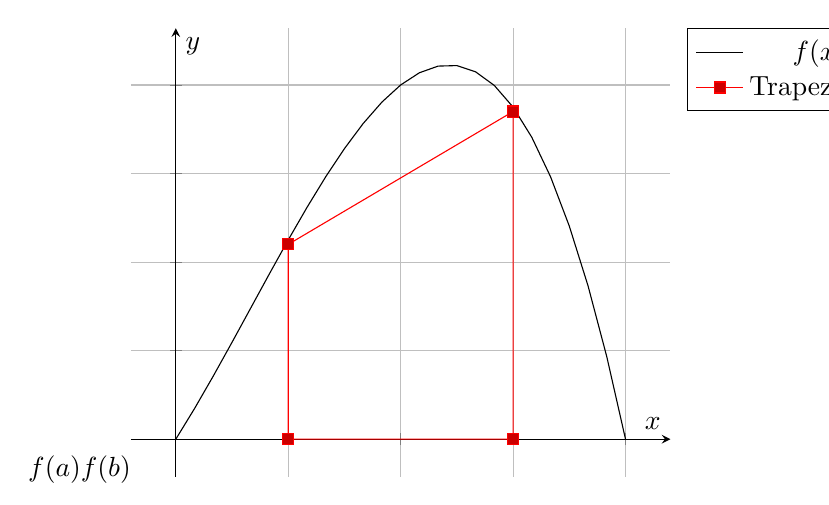
\begin{tikzpicture}
					\begin{axis}[
						axis lines=middle,
						xlabel=$x$,
						ylabel=$y$,
						enlargelimits,
						grid=major,
						xticklabels={,,},
						yticklabels={,,},
						%ymax=2,
						%ymin=-0.5,
						legend pos=outer north east,
						]
						\addplot[domain=0:2] {-1*x^3 + x^2 + 2*x} node[left]{};
						\addplot coordinates {
							( 0.5, 1.1 )
							( 1.5, 1.85 )
							( 1.5, 0)
							( 0.5, 0)
							( 0.5, 1.1)
						};
						\tikzPointLeft{$f(a)$}{0.5,1.1}
						\tikzPointRight{$f(b)$}{1.5,1.85}
						\legend{$f(x)$,Trapezregel}
					\end{axis}
				\end{tikzpicture}
			\caption{Ein zufälliges Beispiel einer Trapezregel. $a$ und $b$ jeweils wie in der Formel rechnet die Trapezregel die umrandete Fläche aus.}
		\end{figure}
	}

	\sbreak
	\bsp{
		\n
		Wir möchten $\int_{1}^{2}f(x) \d x$ einer Funktion $f(x)$ ausrechnen, bei denen wir nur die Stützpunkte $s_0: f(1) = 2$ und $s_1: f(2) = 4$ kennen.
		\\
		Nach der Trapezregel ergibt sich also: 
		\begin{align*} 
 			\QT(f) = 1 \cdot \frac{1}{2} \cdot (2 + 4) = 3 
 		\end{align*}
	}

	\sbreak
	\bsp{
		\n 
		Wir haben die Funktion $f(x) = \sin(x)$. Wir sollen mit den Stellen $x_0 = 0$ und $x_1=\pi$ und der Trapezregel die Fläche in diesen Bereich annähern.
		\begin{align*} 
			\QT(f) &= \pi \cdot 0.5 \cdot (f(0) + f(\pi))\\
				&= \pi \cdot 0.5 \cdot (\sin(0) + \sin(\pi))\\
				&= \pi \cdot 0.5 \cdot (0) \\
				&= 0
		\end{align*}
		Die Trapezregel schätzt, dass die Fläche $0$ ist. Wir wissen aber, dass der Sinus zwischen $0$ und $\pi$ eine Fläche deutlich größer $0$ hat.
		\newpage
		\begin{figure}[H]
			\centering
				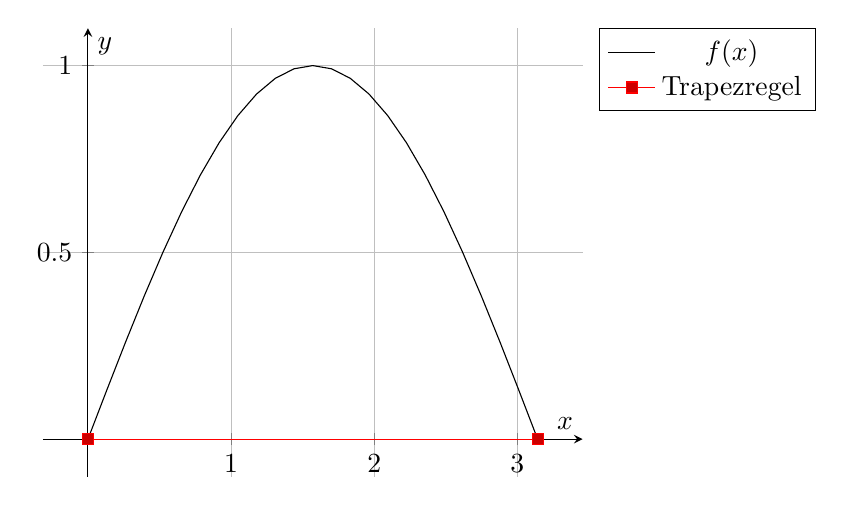
\begin{tikzpicture}
					\begin{axis}[
						axis lines=middle,
						xlabel=$x$,
						ylabel=$y$,
						enlargelimits,
						grid=major,
						ytick={0,0.5,1},
						legend pos=outer north east,
						]
						\addplot[domain=0:pi] {sin(deg(x))} node[left]{};
						\addplot coordinates {
							( 0, 0 )
							( pi, 0 )
						};
						\legend{$f(x)$,Trapezregel}
					\end{axis}
				\end{tikzpicture}
			\caption{Das Problem grafisch. Die Fläche unter dieser Sinuskurve ist definitiv nicht $0$!}
			\label{fig:sinus0}
		\end{figure}
		\noindent Hieran kann man sehen, dass es Fälle gibt, wo die Abschätzung schlecht bis sehr schlecht sein kann.
	}

	\lbreak
	\wichtig{
		\n
		Wir können mit einem Interpolationspolynom vom Grad $2 \cdot n$ ein Polynom vom Grad $2\cdot n+1$ noch exakt integrieren. (ein gerader Grad integriert den nächst höheren ungeraden Grad noch exakt)
	}

	\sbreak
	\bsp{
		\n
		Eine Konstante (Grad 0) kann eine Gerade (Grad 1) exakt integrieren\\
		Aber eine Gerade (Grad 1) kann keine Parabel (Grad 2) exakt integrieren.
	}

	\newpage
	\defi{ \label{defi:quadratur_kondition}
		\n
		Warum erstellt man nicht eine "Regel" mit sehr viel mehr Stützpunkten? 
		\n 
		Das Problem hierbei ist die Kondition. Die entspricht nämlich der Summe aller Beträge der Gewichtungen $\omega$.
		\begin{align} 
 			\sum_i |\omega_i| 
 		\end{align}
		In aller Regel sind die Gewichtungen positiv und ergeben aufaddiert immer 1. Bei Trapezregel ist es $0.5 + 0.5 = 1$, bei Simpsonregel $\nicefrac{1}{6} \cdot (1 + 4 + 1) = 1$ und so weiter.
		Bei deutlich mehr Stützpunkten pro "Regel" (etwa ab 8) werden manche Gewichtungen negativ und somit die Summe der Beträge nicht mehr eins und damit schlechter.
		\n 
		Wir probieren das Problem der Ungenauigkeit auf andere Weise zu verringern. Das behandeln wir im nächsten Kapitel.
	}

	\newpage
	\subsection{Klassische Quadratur}
	\defi{
		\n
		Komplizierte Funktionen liefern meist schlechte Ergebnisse. Die Idee diese zu lösen ist denkbar einfach: Wir wenden die Quadraturregeln stückweise an und unterteilen unser Problem in viele Teilprobleme.
	}

	\sbreak
	\methode{
		\n 
		Beschreibt $H$ den zu integrierenden Bereich (also zwischen $a$ und $b$), $h$ die Länge der einzelnen Stücke, in der wir das Problem aufteilen und $N$ die Anzahl jener. \n
		Formell: 
		\begin{align*} 
 			H &= b - a \aae h = \frac{b-a}{N} \\
			f_i &= f(x_i) \aae x_i = a + i\cdot h 
 		\end{align*}
		\begin{align*} 
 			\QT(f) = H \cdot \frac{f(a) + f(b)}{2} 
 		\end{align*}
		\begin{align} 
 			\rightarrow \QTS(f;h) = h \cdot \l(\frac{f_0}{2} + f_1 + \dots + f_{N-1} + \frac{f_N}{2} \r)
 		\end{align}
		$\QTS$ entspricht dann der \fat{Trapezsumme}.
		\begin{align*} 
			\QS(f) = H \cdot \frac{f(a) + 4 \cdot f\l(\frac{a + b}{2}\r) + f(b)}{6} 
 		\end{align*}
		\begin{align} 
 			\rightarrow \QSS(f;h) = \frac{h}{3}\cdot \l(f_0 + 4f_1 + 2f_2 + 4f_3 + \dots + 2f_{N-2} + 4f_{N-1} + f_N \r)
		\end{align}
		$\QSS$ nennt man die \fat{Simpsonsumme}. Benannt ist dies nach Thomas Simpson.
	}

	\newpage
	\bsp{
		\begin{figure}[H]
			\centering
				\begin{tikzpicture}
					\begin{axis}[
						axis lines=middle,
						xlabel=$x$,
						ylabel=$y$,
						enlargelimits,
						%xticklabels={,,},
						%yticklabels={,,},
						ymax=3.1,
						%ymin=-0.5,
						legend pos=outer north east,
						]
						\addplot[domain=0:2.5] {-1*x^3 + x^2 + 2*x} node[left]{};
						\addplot[dash pattern=on 1pt off 3pt on 3pt off 3pt] coordinates {
							(0.5, 1.1)
							(1, 2)
							(1.5, 1.85)
							(2, 0)
							(2.5, -4.35)
							(2.5, 0)
							(2, 0)
							(1.5, 0)
							(1.5, 1.85)
							(1.5, 0)
							(1, 0)
							(1, 2)
							(1, 0)
							(0.5, 0)
							(0.5, 1.1)
						};
						\addplot[dotted] coordinates {
							(0.5, 0)
							(0.5, 1.1)
							(2.5, -4.35)
							(2.5, 0)
							(0.5, 0)
						};
						\tikzPointLeft{$f(a)$}{0.5,1.1}
						\tikzPointUp{$f(a) + h$}{1,2}
						\tikzPointLeft{$f(b)$}{2.5,-4.35}
						\legend{$f(x)$,Trapezsumme, Trapezregel}
					\end{axis}
				\end{tikzpicture}
			\caption{Beispiel einer Trapezsumme, bei der $N=4$ (in dieser Grafik die gestrichelte Linie) Trapeze konstruiert worden sind, um die Fläche besser anzunähern. Im Vergleich zeigt die gepunktete Linie die Annäherung durch die Trapezregel, also einem Trapez.}
		\end{figure}
	}

	\sbreak
	\bsp{
		\n 
		Und wenn wir uns auch noch einmal das Problem vorher mit Sinus anschauen (siehe \refFigure{fig:sinus0}) sehen wir, dass mehr Trapeze zu einer höheren Genauigkeit führt.
		\begin{figure}[H]
			\centering
				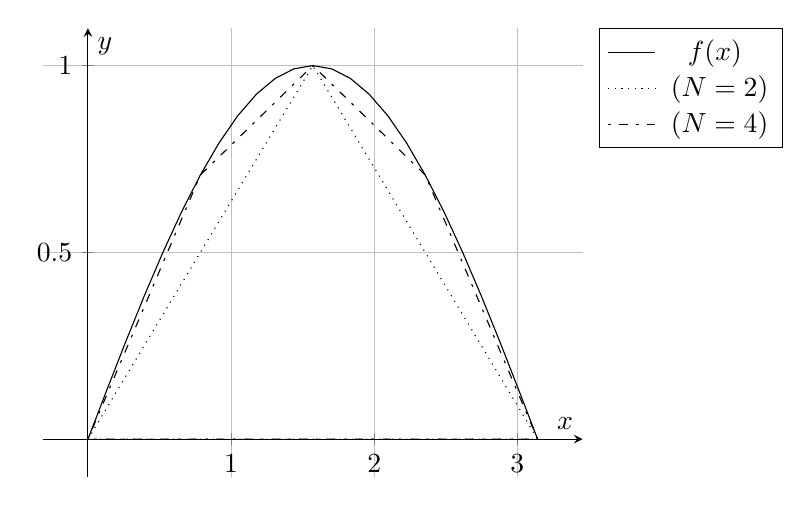
\begin{tikzpicture}
					\begin{axis}[
						axis lines=middle,
						xlabel=$x$,
						ylabel=$y$,
						enlargelimits,
						grid=major,
						ytick={0,0.5,1},
						legend pos=outer north east,
						]
						\addplot[domain=0:pi] {sin(deg(x))} node[left]{};
						\addplot[dotted] coordinates {
							( 0, 0 )
							( pi / 2, 1 )
							( pi, 0 )
							( 0, 0 )
						}; %0.70710678__1186547524400844362104849039284835937688474036588...
						\addplot[dash pattern=on 1pt off 3pt on 3pt off 3pt] coordinates {
							( 0, 0 )
							( pi / 4, 0.70710678 )
							( pi / 2, 1 )
							( (3 * pi) / 4, 0.70710678 )
							( pi, 0 )
							( 0, 0 )
						};
						\legend{$f(x)$, $\QTS$ ($N=2$), $\QTS$ ($N=4$)}
					\end{axis}
				\end{tikzpicture}
			\caption{Die Approximation ist definitiv besser geworden.}
		\end{figure}
	}

	\sbreak
	\subsection{Restglied}

	\defi{
		\n 
		Unter dem sogenannten "Restglied" z.B. einer Trapezsumme beschreibt man die Fehlerabschätzung. Im Grunde also $\RTS \approx \QTS - I(f)$. Diesen Fehler schätzt man nach folgender Formel ab: \n 
		Restglied $\RTS:$ 
		\begin{align} 
 			\RTS(f;h) = h^2 \cdot H \cdot \frac{f^{(2)}(\xi)}{12} 
 		\end{align}
 		Das ganze gibt es dann noch für die Simpsonsumme.
 		\begin{align} 
 			\RSS(f;h) = h^4 \cdot H \cdot \frac{f^{(4)}(\xi)}{180} 
 		\end{align}
 		Das $\xi$ kommt aus dem Mittelwertsatz. Man nimmt hierfür, wenn nötig, meist den Wert aus dem Intervall, dass die Fehlerabschätzung den maximalen Fehler abschätzt und damit den "worst-case".
 		\n 
 		Es ist ziemlich analog zur Fehlerabschätzung einer Polynom-Interpolation, siehe \refChapter{sec:interpolation_fehler}.
	}